\section{Soluzione proposta}
Dopo una attenta lettura ai paper, abbiamo impostato le nostre domande di ricerca, in modo da avere ben chiaro in mente l'obiettivo che volevamo prefiggerci di raggiungere con tale progetto. Le domande al quale tale documento cerca di dare risposta sono le seguenti:
\begin{itemize}
  \item All'interno di una rete sociale come massimizzare il numero di persone che visualizzano una notizia in un numero di step determinato?
  \item Dove è possibile posizionare i bot che generano i contenuti per massimizzare la diffusione ed eventualmente minimizzare il tempo di diffusione?
  \item E' possibile distinguere chi è venuto in contatto con una notizia pubblicata da un determinato tipo di utente (bot o opinion leader) e che informazione possiamo ottenere da tali caratteristiche?
\end{itemize}
Abbiamo scelto quindi la rete di partenza (grafo dei follower del presidente del Consiglio Giuseppe Conte) e da essa abbiamo fatto girare una serie di simulazioni con SOIL. Abbiamo inoltre scelto di seguire le infezioni considerando le differenze tra infetti e esposti e le differenze e per ognuna delle due categorie abbiamo differenziato tra infezione diretta e indiretta, distinguendo anche da chi proviene tale infezione: da bot, da opinion leader o da un altro utente.
\\
Tale progetto è implementato totalmente in Python e i tools e le librerie usate sono le seguenti:
\begin{itemize}
\item Twint: scraper per Twitter;
\item Networkx: per gestire le reti e quindi i grafi;
\item Gephi: per la visualizzazione dei grafi;
\item Plotly: per visualizzare i grafici finali in modo da avere un riscontro visivo dei risultati;
\item Soil: per implementare un modello di simulazione multi-agente;
\item Streamlit: per costruire un'interfaccia grafica in modo da modellare e personalizzare il modello in modo immediato e senza dover passare direttamente dal codice.
\item Pandas: per gestire i dataframe.
\end{itemize}
Siamo quindi partiti da una serie di assunzioni e ipotesi per poi andare a validarle tramite il modello proposto. Tali assunzioni ci hanno guidato nell’impostare il modello, inserendo le probabilità che più ci sembravano vicine alla realtà. Le assunzioni prese in considerazione sono le seguenti:
\begin{itemize}
\item l'Opinion Leader ha influenza maggiore sulla rete rispetto ai Bot;
\item ma i Bot hanno un'influenza più sparsa (ampia);
\item la probabilità di infezione tra utenti è molto bassa;
\item anche la probabilità che l’utente effettui qualche azione (retweet, commento...) dopo essere entrato in contatto con la notizia è bassa e quindi la probabilità di passare da esposto a infetto si alza di molto solo se molti dei suoi vicini hanno risposto a loro volta alla notizia.
\end{itemize}
    \subsection{Grafo}
    \begin{table}[h!]
    \begin{tabular}{ |c|c| }
     \hline
     0-5 & 38353 \\
     \hline
     6-10 & 41 \\
     \hline
     11-20 & 21 \\
     \hline
     21-50 & 34 \\
     \hline
     51-100 & 13 \\
     \hline
     101-250 & 10 \\
     \hline
     251-500 & 12 \\
     \hline
     500+ & 12 \\
     \hline
    \end{tabular}
    \caption{Grafo 500-users}
    \end{table}
    \begin{table}[h!]
    \begin{tabular}{ |c|c| }
     \hline
     0-5 & 105493 \\
     \hline
     6-10 & 80 \\
     \hline
     11-20 & 37 \\
     \hline
     21-50 & 54 \\
     \hline
     51-100 & 35 \\
     \hline
     101-250 & 30 \\
     \hline
     251-500 & 21 \\
     \hline
     500+ & 35 \\
     \hline
    \end{tabular}
    \caption{Grafo 1000-users}
    \end{table}
    \begin{table}[h!]
    \begin{tabular}{ |c|c| }
     \hline
     0-5 & 127327 \\
     \hline
     6-10 & 102 \\
     \hline
     11-20 & 50 \\
     \hline
     21-50 & 67 \\
     \hline
     51-100 & 47 \\
     \hline
     101-250 & 45 \\
     \hline
     251-500 & 27 \\
     \hline
     500+ & 46 \\
     \hline
    \end{tabular}
    \caption{Grafo 1500-users}
    \end{table}
    \begin{table}[h!]
    \begin{tabular}{ |c|c| }
     \hline
     0-5 & 215437 \\
     \hline
     6-10 & 122 \\
     \hline
     11-20 & 64 \\
     \hline
     21-50 & 89 \\
     \hline
     51-100 & 58 \\
     \hline
     101-250 & 57 \\
     \hline
     251-500 & 37 \\
     \hline
     500+ & 57 \\
     \hline
    \end{tabular}
    \caption{Grafo 2000-users}
    \end{table}
    \subsection{Opinion Leader}
    Il social network scelto per effettuare la simulazione è stato Twitter, in particolare è stata scelta la rete sociale dell’attuale presidente del consiglio Giuseppe Conte (username: @GiuseppeConteIT\cite{twitterGiuseppeConte}) che attualmente conta 752.814 follower. Per motivi computazionali non è stato possibile analizzare il grafo completo, quindi sono stati considerati 500 followers e 2 livelli di profondità, per un totale di TODO \\
    Per scaricare i dati necessari, Twitter mette a disposizione delle API ufficiali, ma troppo limitate in termini di richieste per unità di tempo (nella versione standard per ottenere la lista dei followers sono permesse 15 richieste ogni 15 minuti), in particolare avendo la necessità di scaricare informazioni riguardanti migliaia di utenti.\\
    Si è così scelto di usare uno scraper per velocizzare il processo, in particolare è stato usato lo scraper TWINT\cite{Twint} (Twint Intelligence Tool).
    \subsection{Bot}\label{Bot}
    Per determinare la posizione dei Bot all'interno della rete sono state calcolate le principali misure di centralità dei nodi all'interno del grafo, basate su:
    \\
    \textbf{In-Degree}
    \\
    Numero di archi entranti di un nodo, misura quanto un utente è seguito.\\
    Formalmente:

    \\
    \textbf{Betweenness}
    \\
    Numero di volte che un nodo funge da ponte lungo il percorso più breve tra 2 nodi; su una rete sociale corrisponde a quanto un utente si trova sui percorsi di comunicazione tra gli altri utenti.\\
    Formalmente:

    \\
    \textbf{Autovettori}
    \\
    Misura l'importanza di un nodo, un nodo è considerato importante se puntato da altri nodi importanti. \\
    Formalmente:
    \\
    É stata inoltre, svolta una simulazione considerando una posizione randomica dei Bot.

    \subsection{Simulazioni}
    Durante le simulazioni è stato selezionato come Opinion Leader l’esatto nodo che, all’interno del grafo ottenuto grazie allo scraper, rappresenta il Presidente del Consiglio. I Bot all’interno delle simulazioni sono sempre 10 tuttavia differiscono per la loro posizione all’interno della rete. Poiché gli stessi nodi con in-degree maggiore sono gli stessi con betweenness maggiore allora la simulazione sarà unica. Si avranno quindi tre simulazioni:
    \begin{itemize}
    \item Simulation_BTW: simulazione nella quale i nodi selezionati come Bot sono posti nei nodi aventi betweenness maggiore.
    \item Simulation_Eigenvector: simulazione nella quale i nodi selezionati come Bot sono i 10 nodi considerati più influenti sulla base degli eigenvector score.
    \item Simulation_Random: simulazione nella quale i nodi selezionati come Bot sono presi in modo random.
    \end{itemize}
    \subsection{Configurazione di SOIL}\label{ConfigSoil}

        \subsubsection{File Python}
        Nel file PY viene descritto il modulo python che verrà poi usato per avviare la simulazione seguendo le direttive e le caratteristiche descritte nel file YML. Per ogni agente viene quindi creata una classe la quale avrà degli stati e dei metodi che ne descrivono i comportamenti e interazioni tra i vari agenti. Nel nostro caso ci sono 3 tipologie di agenti:
        \begin{itemize}
        \item OpinionLeader: è l’utente dal quale è stato generato il grafo e da cui tramite scraper si sono ottenuti i suoi follower e poi i follower dei follower. Nel nostro caso è l’utente Conte.
        \item Bot: sono i bot che hanno interesse a far espandere una notizia pubblicando spesso contenuti, hanno quindi un potere di influenza mediamente alto. La selezione di questi bot viene effettuata nel file BotSelection.py, tale selezione può avvenire sulla base dei parametri descritti nella sezione ~\ref{Bot}.
        \item User: sono gli utenti comuni, possono trovarsi in tre stati:
          \begin{itemize}
          \item not_exposed: l’utente non è entrato per niente in contatto con una determinata notizia o informazione, nè perchè è stato esposto nè guardando la home di tweeter o cercando manualmente (quest’ultima casistica è gestita dal campo prob_search_spread).
          \item exposed: l’utente è entrato in contatto con la notizia ma non ha ancora effettuato nessuna azione,quindi non ha mostrato agli altri della sua rete di essere entrato in contatto con tale informazione.
          \item infected: l’utente non solo è stato esposto ma ha anche palesato il suo essere entrato in contatto con la notizia effettuando un'azione e quindi potenzialmente è in una condizione in cui potrebbe esporre altri utenti.
          \end{itemize}
        \end{itemize}
        All’inizio della simulazione i soli che sono considerati esposti sono l’opinion leader e i bot dai quali appunto si propaga l’informazione. Per una questione di maggior controllo dei risultati finali, e quindi per vedere chi e quanto ha contribuito alla propagazione, è stato introdotto un parametro type. Quest’ultimo ha valore 1 nel caso la propagazione è partita dall’opinion leader, 2 nel caso avviene dai bot; utenti infettati da altri utenti propagano comunque il tipo da cui sono stati infettati, e quindi ad esempio un utente infettato da un utente che era stato in principio infettato da un bot avrà tipo 2 e sarà quindi conteggiato tra quelli infettati dai bot.
        \subsubsection{File YML}
        Il file YML racchiude le specifiche delle simulazioni che saranno lanciate con soil.\\
        Tra i parametri personalizzabili particolarmente utili sono:
        \begin{itemize}
          \item max_time: numero di step effettuati al massimo nella simulazione.
          \item num_trials: parametro tramite il quale si può decidere se rifare la stessa simulazione più volte indicando il numero di volte che sarà lanciata.
          \item network_params: parametro nel quale si seleziona il grafo su cui sarà effettuata la simulazione, può essere o creato in maniera random o preso da un grafo già creato indicando il file GEXF.
          \item states: parametro che permette di personalizzare il singolo nodo tramite il suo id. Ciò ci ha permesso di selezionare la posizione sempre fissa di Conte e di verificare come le simulazioni cambiassero in base alla marcatura di alcuni nodi come Bot sulla base di dei parametri specifici, indicati nella sezione ~\ref{Bot}.
        \end{itemize}

    \subsection{Web app}
      Per ragioni di riproducibilità più agevole e per estensibilità è stato scelto di sviluppare una web app che permettesse l’esecuzione di tutte le fasi contemplate dall’app e anche di ottenere i risultati in forma di grafici.\\
      Per lo sviluppo della webapp è stata usata la libreria streamlit. Streamlit è un framework open-source in Python. E’ particolarmente utile per data scientists e sviluppatori che lavorano nel campo di machine learning.\\

      Di seguito si illustrano le varie fasi dell’app.
        \subsubsection{Fasi dell'app}
          \\
          \textbf{Download dati da Twitter}
          \\
          In questa fase abbiamo utilizzato lo scraper TWINT per ottenere i followers di Conte e, a loro volta, i followers dei followers di Conte. Il risultato ottenuto è un file .csv per ogni utente di Twitter, all'interno del quale sono segnati gli user dei followers.
          \\
          \textbf{Creazione del grafo}
          \\
          Da questi file .csv ottenuti dalla fase precedente, si è creato il grafo orientato (secondo la relazione di “Follow”) tramite la libreria networkx.
          \\
          \textbf{Posizionamento Bot e simulazione SOIL}
          \\
          Oltre a configurare e far eseguire le simulazioni di soil, così come spiegato nella sezione ~\ref{ConfigSoil}, in tale fase sono state effettuate le principali misure di centralità dei nodi nel grafo in modo da determinare la posizione dei Bot, ed effettuate le simulazioni appropriate.
          \\
          \textbf{Visualizzazione grafo risultante}
          \\
          In questa fase vengono mostrati i risultati delle simulazioni in forma di grafo. I nodi del grafo sono stati colorati differentemente a seconda dello stato dell’agente corrispondente (non esposto, esposto, infetto), inoltre, viene riportato anche il tipo di nodo che ha causato la diffusione/contagio.
          \\
          \textbf{Statistiche sulla diffusione}
          \\
          A questo punto abbiamo provveduto a calcolare le statistiche ottenute dai risultati, andando a calcolare le percentuali dei non esposti, esposti, infetti, per ogni fase e da chi sono stati infettati o esposti (bot, user, opinion leader).
        \subsubsection{Uso di streamlit}
          L'app è strutturata con un pannello di configurazione a sinistra.
          \begin{figure}[H]
              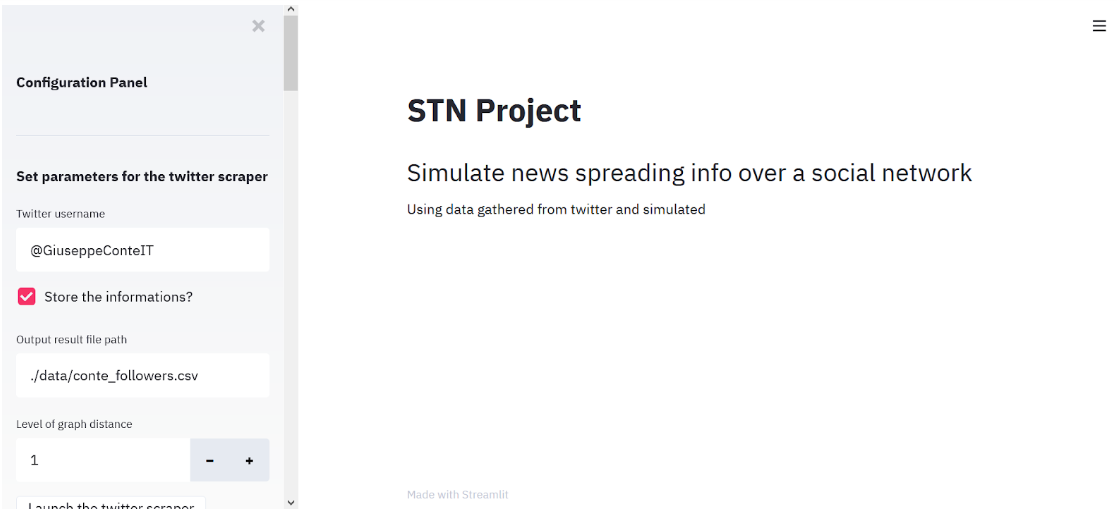
\includegraphics[width=16cm]{resources/panelApp.png}
              \caption{Screen dell'app}
          \end{figure}
          Da tale pannello è possibile:
          \begin{itemize}
            \item Scegliere i parametri per il twitter scraper:
              \begin{itemize}
                \item Scegliere lo username dell'account su cui avviare lo scraper.
                \item Salvare il csv ottenuto.
                \item Selezionare il path nel quale salvare il csv contenente i follower dell'account scelto.
                \item Specificare a che livello scendere nel grafo dei follower (1 o 2).
              \end{itemize}
            \item Parametri per generare il grafo:
              \begin{itemize}
                \item Selezionare il path da cui prendere le informazioni (csv).
                \item Selezionare la cartella da cui prendere il secondo livello del grafo (se presente).
                \item Scegliere il nome del grafo.
                \item Selezionare se salvare il grafo come diretto o indiretto.
                \item Numero di follower da considerare.
              \end{itemize}
            \item Parametri per la selezione dei Bot:
              \begin{itemize}
                \item Path del grafo (.gexf).
                \item Selezione del metodo con cui calcolare i bot.
                \item Selezionare il numero dei bot da inserire nella rete.
              \end{itemize}
            \item Parametri per la simulazione di SOIL:
              \begin{itemize}
                \item Path del file yml a partire dal quale configurare la simulazione.
                \item Scegliere il nome della simulazione.
                \item Selezionare il path della cartella principale dedicata alle simulazioni.
                \item Scegliere il numero massimo di iterazioni della simulazione.
                \item Scegliere il numero di volte che la simulazione sarà lanciata con quei parametri.
                \item Selezionare il file gexf contenente le caratteristiche del grafo.
              \end{itemize}
            \item Parametri per la creazione dei grafici e dei risultati:
              \begin{itemize}
                \item Selezione del file del grafo di partenza (.gexf).
                \item File csv contenente l’output della simulazione di SOIL.
                \item Nome della simulazione, sulla base della tipologia di selezione dei bot (random, btw o eigenvector).
                \item Numero di step effettuati durante la simulazione sul grafo.
                \item Visualizzare o no graficamente il grafo.
              \end{itemize}
            \item Parametri per calcolare le statistiche finali:
              \begin{itemize}
                \item Nome della simulazione, sulla base della tipologia di selezione dei bot (random, btw o eigenvector).
                \item Numero di step effettuati durante la simulazione sul grafo.
              \end{itemize}
          \end{itemize}
